\documentclass{article}

\usepackage{geometry}
\usepackage{afterpage}
\usepackage{graphicx}
\usepackage{outlines}
\usepackage{hyperref}
\usepackage{changepage}
\usepackage{amssymb}
\usepackage{amsfonts}
\usepackage{pdflscape}
\usepackage{amsmath}
\usepackage{amsthm}
\usepackage{blindtext}

\author{Astrid Augusta Yu}
\title{CSC 348 -- Homework \#5}
\date{\today}

\newcommand{\contradiction}{$\rightarrow\leftarrow$}
\renewcommand\qedsymbol{\texttt{d(\textbf{\^{}\_\^{}})>}}
\newtheorem{theorem}{Theorem}
\newtheorem{lemma}{Lemma}
\newtheorem{case}{Case}
\newtheorem{subcase}{Case}
\numberwithin{subcase}{case}

\begin{document}
\maketitle
\tableofcontents

\section{Questions}
\begin{outline}[enumerate]
    \1 \begin{theorem}
        For all $n \in \mathbb{Z}^+$, $133$ divides $11^{n+1} + 12^{2n-1}$
    \end{theorem}
    \begin{proof}
        Let the sequence $a_n = 11^{n+1} + 12^{2n-1}$. We will first rewrite it 
        recursively.

        \textbf{Base case.}
        \begin{equation}
            \begin{aligned}
                a_1 &= 11^{1+1} +12^{2\cdot 1 - 1} \\
                &= 11^2 + 12^1  \\
                &= 133
            \end{aligned}
            \label{eqn:133-recb}
        \end{equation}

        \textbf{Recursive step.} We can derive the recursive step by transforming $a_{n+1} - a_n$ using the 
        explicit definition of $a_n$.
        \begin{equation}
            \begin{aligned}
                a_{n+1}-a_n &= 11^{n+2} + 12^{2n+1} - \left(11^{n+1} + 12^{2n-1}\right)  \\
                &= 11\cdot 11^{n+1} + 144\cdot 12^{2n-1} - 11^{n+1} - 12^{2n-1}  \\
                &= (11 - 1)\cdot 11^{n+1} + (144 - 1)\cdot 12^{2n-1}  \\ 
                &= 10\cdot 11^{n+1} + 143\cdot 12^{2n-1}  \\
            \end{aligned}
            \label{eqn:133-rec1}
        \end{equation}

        We can further rearrange the equation like so:        
        \begin{equation}
            \begin{aligned}
                a_{n+1}&= a_n + 10\cdot 11^{n+1} + 143\cdot 12^{2n-1}  \\
                &= a_n + 10\cdot 11^{n+1} + 10\cdot 12^{2n-1} + 133\cdot 12^{2n-1}\\
                &= a_n + 10\cdot \left(11^{n+1} + 12^{2n-1}\right) + 133\cdot 12^{2n-1}\\
            \end{aligned}
            \label{eqn:133-rec2}
        \end{equation}

        We can substitute the explicit definition of $a_n$ into (\ref{eqn:133-rec2}) like so:
        \begin{equation}
            \begin{aligned}
                a_{n+1}&= a_n + 10 a_n + 133\cdot 12^{2n-1}\\
                &= 11 a_n + 133\cdot 12^{2n-1}\\
            \end{aligned}
            \label{eqn:133-rec3}
        \end{equation} 

        Thus, we have our recursive definition of $a_n$:
        \begin{equation}
            \begin{aligned}
                a_1 &= 133 \\ 
                a_{n+1} &= 11 a_n + 133\cdot 12^{2n-1}\\
            \end{aligned}
            \label{eqn:133-recdef}
        \end{equation}

        Now, we will use this to prove $133\ |\ a_n$ by induction.

        \textbf{Base case.} Consider when $n = 1$. By (\ref{eqn:133-recdef}), $a_1 = 133$. Thus, 
        $133\ |\ a_1$ is equivalent to $133\ |\ 133$, which is obviously true.

        \textbf{Inductive hypothesis.} Consider when $n = k$. Suppose that $133\ |\ a_k$. This implies 
        that there exists some $i \in \mathbb{Z}$ such that $a_k = 133i$.

        \textbf{Inductive step.} Consider when $n = k + 1$. By (\ref{eqn:133-recdef}):
        \begin{equation}
            a_{k+1} = 11 a_k + 133\cdot 12^{2k-1}
        \end{equation}

        By the inductive hypothesis, we can substitute $a_k = 133i$ in and rearrange:
        \begin{equation}
            \begin{aligned}
                a_{k+1} &= 11 \cdot (133i) + 133\cdot 12^{2k-1} \\
                &= 133\cdot\left(11 \cdot i + 12^{2k-1}\right) \\
            \end{aligned}
        \end{equation}

        Let $j=11 \cdot i + 12^{2k-1}$. Then, $a_{k+1} = 133j$. Therefore, $133\ |\ a_{k+1}$.

        Thus, by the principle of mathematical induction, $133\ |\ a_n$, and $133\ |\ 11^{n+1} + 12^{2n-1}$.

    \end{proof}

    \1 \begin{theorem}
        For all $n \in \mathbb{N}^+$ there exists $a \in \mathbb{N}^+_{odd}$ and $b \in \mathbb{N}$ such that $n = a\cdot 2^b$.
    \end{theorem}

    \begin{proof}
        \textbf{Base case.} Consider $n = 1$. Select $a = 1$ and $b = 0$: 
        \begin{equation}
            n = 1 = a\cdot 2^b = 1 \cdot 2^0 = 1
        \end{equation}
        Thus, the theorem applies for $n = 1$.

        Additionally, consider $n = 2$. Select $a = 1$ and $b = 1$: 
        \begin{equation}
            n = 2 = a\cdot 2^b = 1 \cdot 2^1 = 2
        \end{equation}
        Thus, the theorem applies for $n = 2$.

        \textbf{Inductive hypothesis.} Suppose that for all $1 \leq n < k$, there exists $a_n \in \mathbb{N}^+_{odd}$ and $b_n \in \mathbb{N}$ such that 
        \begin{equation}
            n = a_n \cdot 2^{b_n}
            \label{eqn:a2b-ih}            
        \end{equation}

        \textbf{Inductive step.} Consider $n = k$. 

        \begin{adjustwidth}{0.5cm}{0cm}
            
            \textbf{Case 1.} Consider the case when $k$ is even. Let $i \in \mathbb{Z}$ such that $k = 2i$.

            Since $i < k$, by the induction hypothesis, there exists some $2j + 1 \in \mathbb{N}^+_{odd}$ 
            and $c \in \mathbb{N}$ such that
            \begin{equation}
                i = (2j+1) \cdot 2^c
                \label{eqn:a2b-odd-ev-ih}
            \end{equation}

            Multiplying both sides by $2$ yields a definition for $k$:
            \begin{equation}
                \begin{aligned}                
                    2i = k &= 2\cdot (2j+1) \cdot 2^c \\
                    &= (2j+1) \cdot 2^{c + 1} \\
                \end{aligned}
                \label{eqn:a2b-post-ih}
            \end{equation}

            Suppose $a = 2j + 1$ and $b = c + 1$. Therefore, 
            \begin{equation}
                k = a\cdot 2^b
            \end{equation}

            Thus, for all $n \in \mathbb{N}^+_{even}$ there exists $a \in \mathbb{N}^+_{odd}$ and $b \in \mathbb{N}$ such that $n = a\cdot 2^b$.

            \textbf{Case 2.} Consider the case when $k$ is odd. 
            \begin{equation}
                k = k \cdot 1 = k \cdot 2^0
            \end{equation}

            Let $a = k$ and $b = 0$. Thus, 
            \begin{equation}
                k = a \cdot 2^b
            \end{equation}

            Thus, for all $n \in \mathbb{N}^+_{odd}$ there exists $a \in \mathbb{N}^+_{odd}$ and $b \in \mathbb{N}$ such that $n = a\cdot 2^b$.

        \end{adjustwidth}
            
        Since \textbf{Case 1} and \textbf{Case 2} are true, this covers all the cases for 
        $n \in \mathbb{N}^+$. 

        Therefore, by the principle of strong mathematical induction, for all $n \in \mathbb{N}^+$ there 
        exists $a \in \mathbb{N}^+_{odd}$ and $b \in \mathbb{N}$ such that $n = a\cdot 2^b$.

    \end{proof}

    \1 \begin{theorem}
        Let $f_n$ be the $n$th Fibonacci number. For all $n \in \mathbb{Z}^+$, $\sum^{n}_{i=1} f_i^2 = f_nf_{n+1}$
    \end{theorem}

    \begin{proof}
        \textbf{Base case.} Consider $n = 1$. 
        \begin{equation}
            \sum^{1}_{i=1} f_i^2 = f_1^2 = 1^2 = 1           
        \end{equation}

        \begin{equation}
            f_1f_2 = 1\cdot 1 = 1
        \end{equation}

        Therefore, $\sum^{n}_{i=1} f_i^2 = f_nf_{n+1}$ for $n = 1$.

        \textbf{Inductive hypothesis.} Suppose that for some $k \in \mathbb{Z}^+$,

        \begin{equation}
            \sum^{k}_{i=1} f_i^2 = f_kf_{k+1}
        \end{equation}

        \textbf{Inductive step.} Consider the case when $n = k + 1$.

        \begin{equation}
            \sum^{k + 1}_{i=1} f_i^2 = f_{k+1}^2 + \sum^{k}_{i=1} f_i^2
        \end{equation}

        By the inductive hypothesis, this expression is equivalent to
        \begin{equation}
            f_{k+1}^2 + f_k f_{k + 1} = f_{k + 1}\left(f_{k + 1} + f_k\right)
        \end{equation}

        By definition of the Fibonacci sequence, $f_{k + 1} + f_k = f_{k+2}$. Substituting into 
        the equation:
        \begin{equation}
            f_{k + 1}f_{k+2} = f_{(k + 1)}f_{(k + 1) + 1}
        \end{equation}

        Therefore, for all $n \in \mathbb{Z}^+$, $\sum^{n}_{i=1} f_i^2 = f_nf_{n+1}$.

    \end{proof}

    \1 \begin{theorem}
        Let $f_n$ be the $n$th Fibonacci number. For all $n \in \mathbb{Z}^+$, $\sum^{n}_{i=1} f_{2i-1} = f_{2n}$.
    \end{theorem}

    \begin{proof}
        \textbf{Base case.} Consider $n = 1$. 
        \begin{equation}
            \sum^{1}_{i=1} f_{2i-1} = f_{2\cdot 1 - 1} = f_1 = 1
        \end{equation}

        \begin{equation}
            f_{2\cdot 1} = f_2 = 1
        \end{equation}

        Therefore, $n \in \mathbb{Z}^+$, $\sum^{n}_{i=1} f_{2i-1} = f_{2n}$ for $n = 1$.

        \textbf{Inductive hypothesis.} Suppose that for some $k \in \mathbb{Z}^+$,

        \begin{equation}
            \sum^{k}_{i=1} f_{2i-1} = f_{2k}
        \end{equation}

        \textbf{Inductive step.} Consider the case when $n = k + 1$.

        \begin{equation}
            \begin{aligned}
                \sum^{k+1}_{i=1} f_{2i-1} &= f_{2(k+1)-1} + \sum^{k}_{i=1} f_{2i-1} \\
                &= f_{2k+1} + \sum^{k}_{i=1} f_{2i-1}
            \end{aligned}
        \end{equation}

        By the inductive hypothesis, this expression is equivalent to
        \begin{equation}
            f_{2k+1} + f_{2k}
        \end{equation}

        By definition of the Fibonacci sequence, $f_{2k+1} + f_{2k} = f_{2k+2}$. Substituting into 
        the equation:
        \begin{equation}
            f_{2k+2} = f_{2(k+1)}
        \end{equation}

        Therefore, for all $n \in \mathbb{Z}^+$, $\sum^{n}_{i=1} f_{2i-1} = f_{2n}$.

    \end{proof}

    \1 For each of the following definitions of $a_n$, show $(a_n)^3_{n=0}$
        \2 $(1, -2, 4, -8)$
        \2 $(3, 3, 3, 3)$
        \2 $(8, 11, 23, 71)$
        \2 $(2, 0, 8, 0)$
    \1 For each of the following definitions of $a_n$, show $\sum^3_{n=0}a_n$
        \2 $-5$
        \2 $12$
        \2 $113$
        \2 $10$

    \1 Consider the sequence $a_i = i^2$.
        \2 $(a_i)^3_{i=0} = (0, 1, 4, 9)$
        \2 $\sum^3_{i=0} a_i = (0, 1, 5, 14)$
        \2 $s = (a_i)^n_{i=0}$ is a $n + 1$ element sequence that looks like
        $$(0, 1, 4, 9, \dots, (n-3)^2, (n-2)^2, (n-1)^2, n^2)$$
        
        Assuming $s$ is 1-indexed, the $j$th element of $s$ is $(j-1)^2$.

    \1 $(a_n)^4_{n=0} = (0, 2, 5, 33, 8589934593)$

    \1 
        \2 \begin{equation}
            \begin{aligned}
                \text{Basis step}&& a_0 &= 0 \\
                \text{Recursive step}&& a_n &= a_{n-1} + 2
            \end{aligned}
        \end{equation}
        \2 \begin{equation}
            \begin{aligned}
                \text{Basis step}&&a_0 &= 1 \\
                \text{Recursive step}&&a_n &= a_{n-1} + 2
            \end{aligned}
        \end{equation}
        \2 \begin{equation}
            \begin{aligned}
                \text{Basis step}&&1 &\in S \\
                \text{Recursive step}&&x \in S &\rightarrow 3x \in S
            \end{aligned}
        \end{equation}
    
    \1 
        \2 \begin{equation}
            \begin{aligned}
                \text{Basis step}&& a_1 &= 6  \\
                \text{Recursive step}&& a_n &= a_{n-1} + 6
            \end{aligned}
        \end{equation}
        \2 \begin{equation}
            \begin{aligned}
                \text{Basis step}&& a_1 &= 3  \\
                \text{Recursive step}&& a_n &= a_{n-1} + 2
            \end{aligned}
        \end{equation}
        \2 \begin{equation}
            \begin{aligned}
                \text{Basis step}&& a_1 &= 10 \\
                \text{Recursive step}&& a_n &= 10a_{n-1}
            \end{aligned}
        \end{equation}
        \2 \begin{equation}
            \begin{aligned}
                \text{Basis step}&& a_1 &= 5 \\
                \text{Recursive step}&& a_n &= a_{n-1}
            \end{aligned}
        \end{equation}
    
    \1 
        \2 Step 0: $\{(0, 0)\}$
        
        Step 1: $\{(0, 0), (2, 3), (3, 2)\}$
    
        Step 2: $\{(0, 0), (2, 3), (3, 2), (4, 6), (5, 5), (6, 4)\}$
    
        Step 3: $\{(0, 0), (2, 3), (3, 2), (4, 6), (5, 5), (6, 4), (6, 9), (7, 8), (8, 7), (9, 6)\}$

        \2 $$S = \left\{ (x, y) \in \mathbb{N}^2\ |\ a, b \in \mathbb{N} \wedge x = 3a + 2b \wedge y = 2a + 3b \right\}$$

        \2 \begin{theorem}
            If $(a, b) \in S$ then $5\ |\ (a + b)$.
        \end{theorem}

        \begin{proof}
            \textbf{Base case.} Suppose $(a, b) = (0, 0)$. Thus, $5\ |\ (0 + 0) \equiv 5\ |\ 0$, which is 
            true because everything divides $0$.

            \textbf{Inductive hypothesis.} Suppose $(a, b) \in S$ and $5\ |\ (a + b)$. 

            It follows that for some $i \in \mathbb{Z}$, 
            \begin{equation}
                5i = a + b
            \end{equation}

            \textbf{Inductive step.} 
            By the inductive hypothesis $(a, b) \in S$.
            
            Therefore, it follows that $(a + 3, b + 2),(a + 2, b + 3) \in S$. WLOG, consider 
            the case for $(a + 3, b + 2) \in S$.

            $$(a + 3) + (b + 2) = a + b + 5$$

            By the inductive hypothesis, this expression is equal to 

            $$5i + 5 = 5(i + 1)$$

            Let $j = i + 1$. Thus, 

            $$(a + 3) + (b + 2) = 5j$$

            By definition of divides, $5\ |\ \left[(a + 3) + (b + 2)\right]$.

            Therefore, by the principle of mathematical induction, for all $(a, b) \in S$, 
            $5\ |\ (a + b)$. 
        \end{proof}
    
\end{outline} 


\newgeometry{margin=2cm}
\begin{landscape}
    \section{Scratch Work}

    \centering
    \thispagestyle{empty}
    \includegraphics[width=0.95\linewidth]{1.jpg}

    \pagebreak
    
    \thispagestyle{empty}
    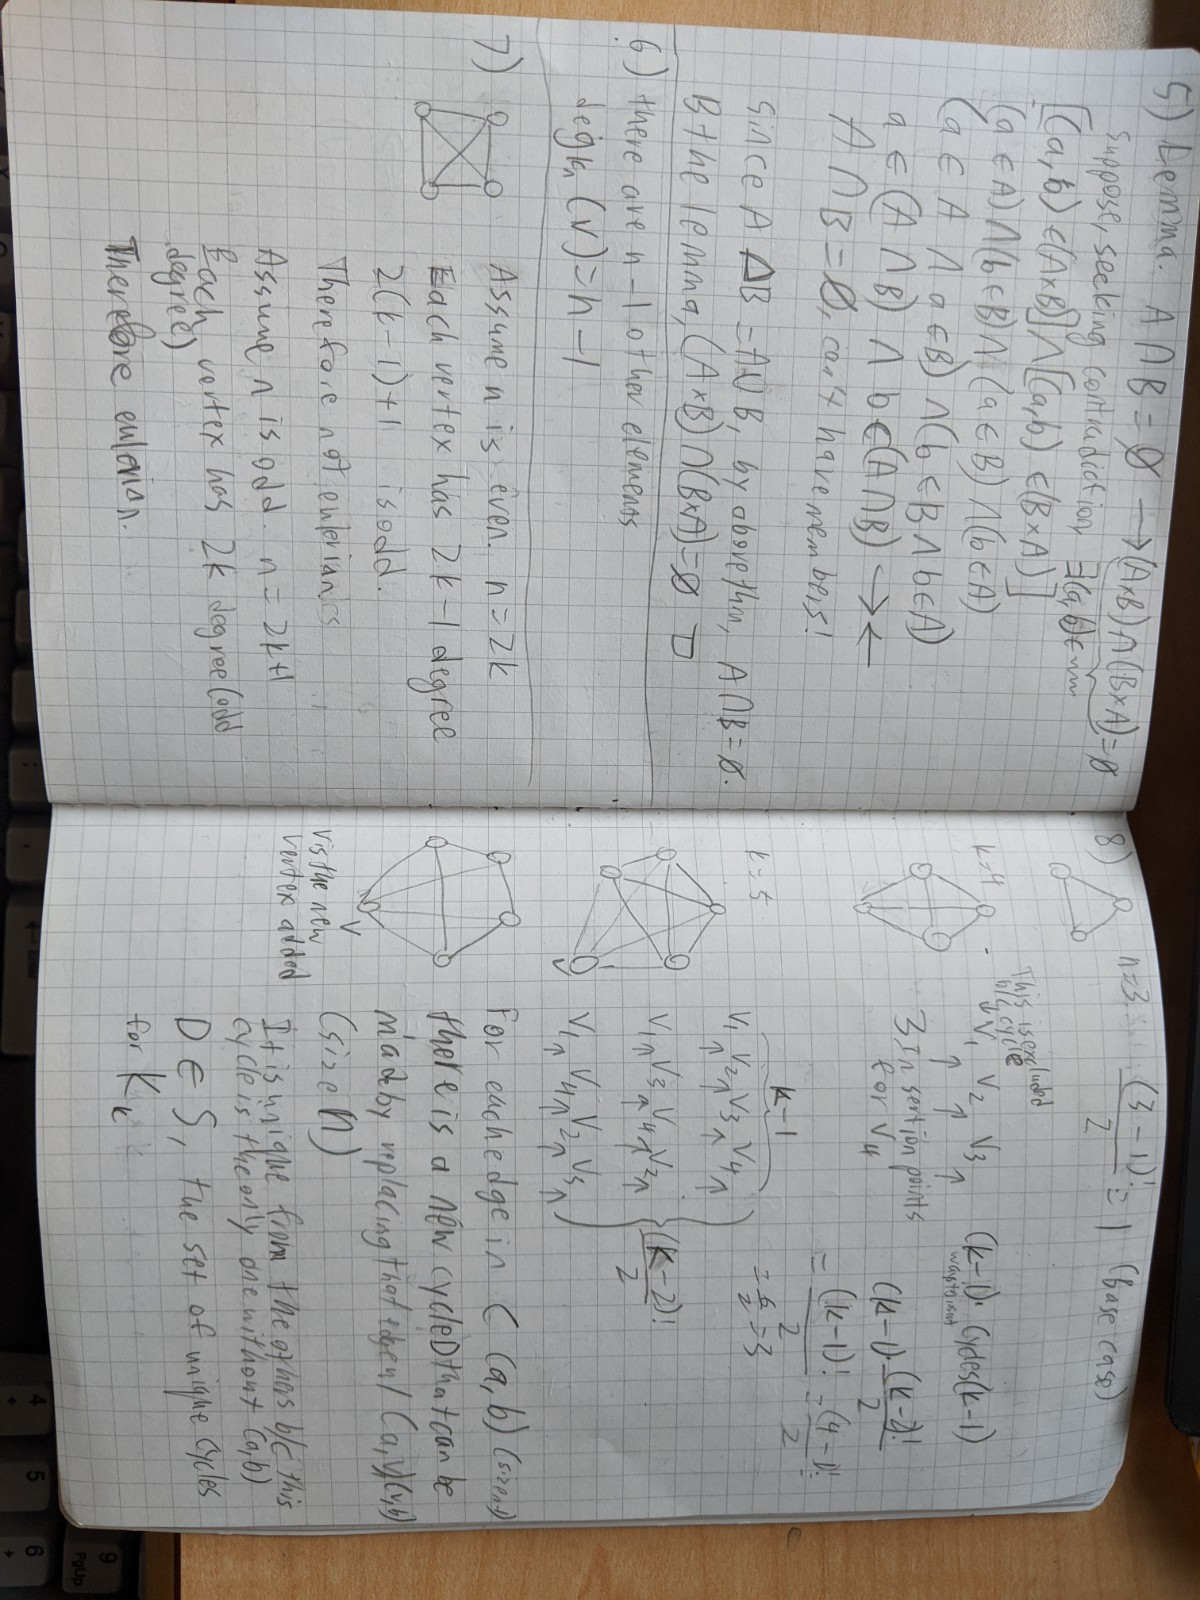
\includegraphics[width=0.95\linewidth]{2.jpg}
    \pagebreak
    
    \thispagestyle{empty}
    \includegraphics[width=0.95\linewidth]{3.jpg}
    \pagebreak
    
    \thispagestyle{empty}
    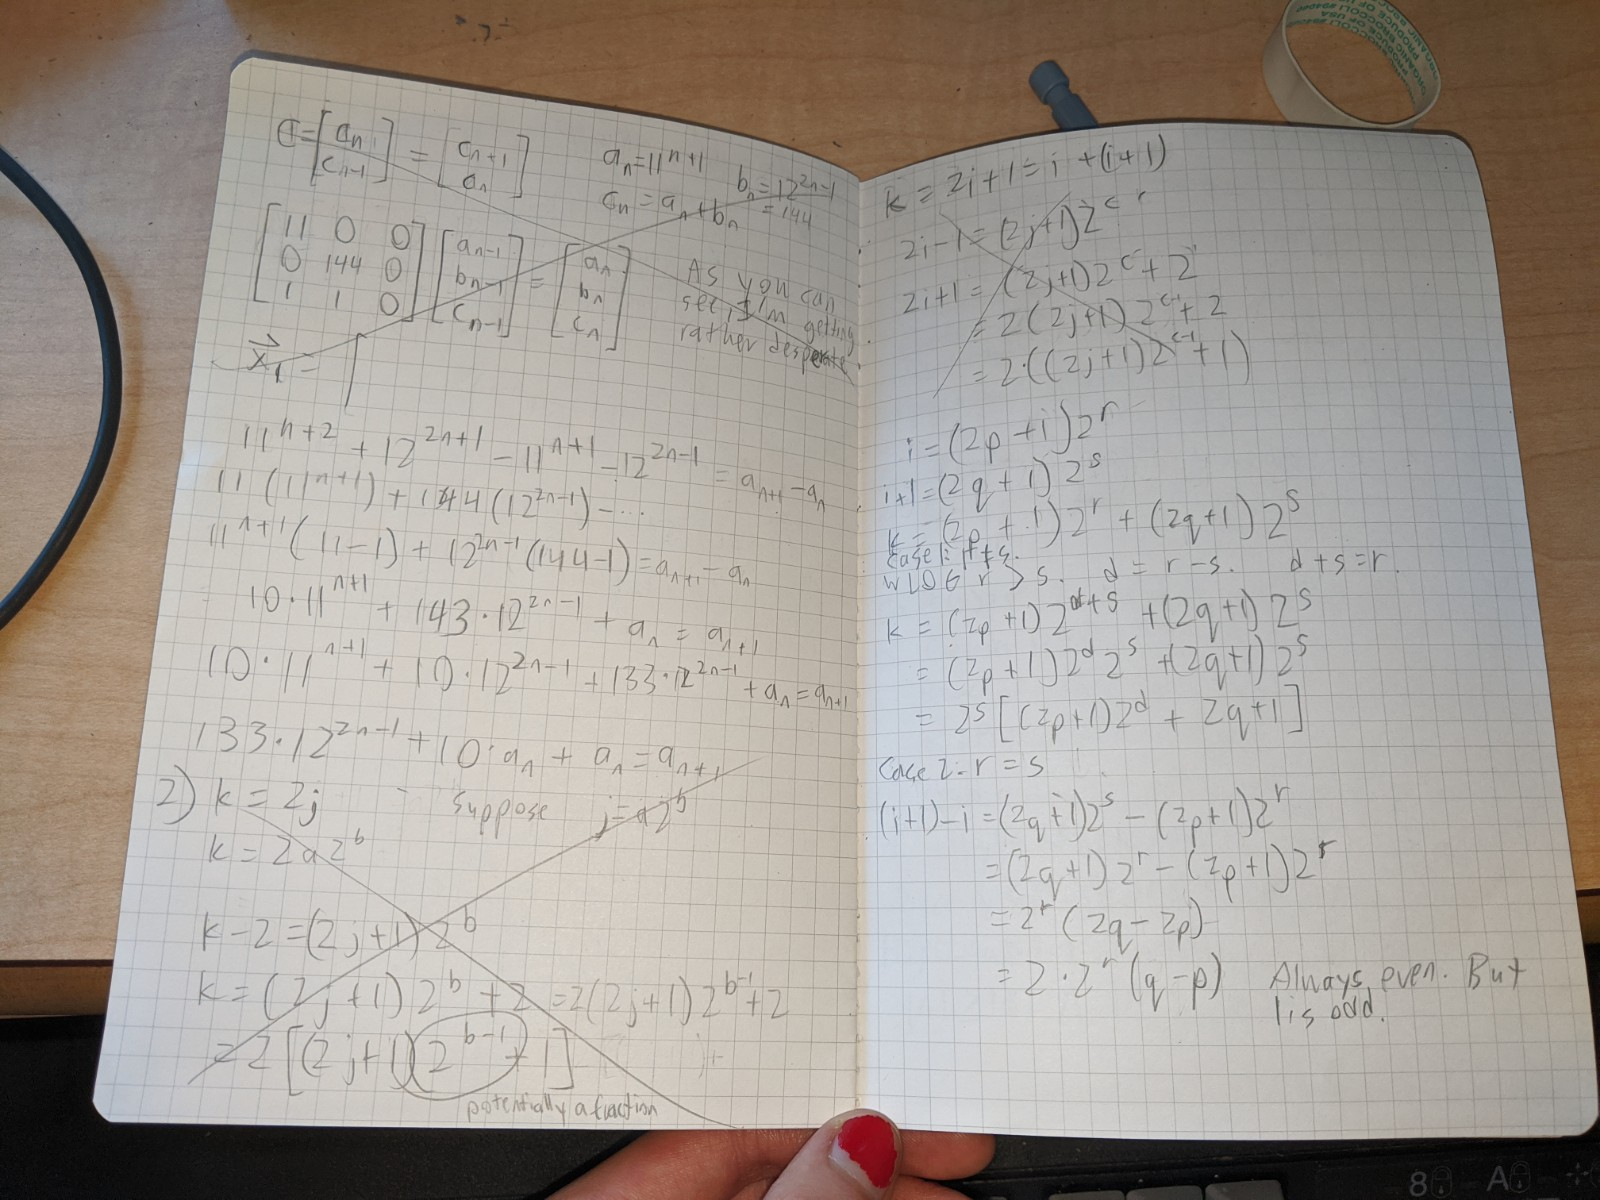
\includegraphics[width=0.95\linewidth]{4.jpg}
\end{landscape}

\restoregeometry
    
\end{document}